\cotefile{14}
\scanpage{2}
\deleted{Les \unsure{éléments} de \unsure{structure} motiviques \& leur interprétation en \unsure{termes} de \unsure{groupes} algébriques sur $\mathbb{Q}$}

\uline{Structure d'effectivité}

\mspage{1}


\scanpage{3}
Structure

\unsure{4}$^\circ$) La donnée d'une sous-catégorie \inserted{\unsure{str.$^{\mathrm t}$} pleine} de $M$ (motifs effectifs), \unsure{stabl.} pr $\otimes$, pr sommes, \deleted{\unsure{quotients}} pr sous-\deleted{\unsure{tout}}objets, telle que \inserted{où $\Lambda(-1)$ soit effectif et que} pour $\forall E$, $\exists$ entier $n$ tel que $E(-n)\inserted{{}=E\otimes\Lambda(-1)^{\otimes n}}$ soit ``effectif''. Une telle structure sur $G_{\unsure{\mathbb{Q}}}$ en définit une \unsure{analogue} sur $G_{\mathbb{C}}$, et réciproqt; donc une telle notion de structure peut être considérée comme équivalente à la donnée d'un
\deleted{\unsure{partie de} $\unsure{K^+}(G)$ \unsure{bon cône}}
\deleted{cône $\unsure{X^+}$, $K^+(G)$}
\inserted{cône $K^+(G)$}
\deleted{\unsure{l'anneau} \unsure{des caractères} de $G_{\unsure{\mathbb{Q}}}$ $(\unsure{X^+}+\unsure{X^+}\subset\unsure{X^+})$}
\deleted{$\unsure{\Lambda}$ \unsure{stabl.} pr produit, tel que \unsure{pour tout}}
dans \inserted{l'anneau des car. sur $\mathbb{Q}$,} $K(G)$, contenant $0$, \deleted{$\unsure{1}$} $\varepsilon$, stable pr multiplication, et $\unsure{\lambda|\Lambda}$. À priori, on \unsure{aurait|devrait} là une notion de structure faisant intervenir la structure sur $\mathbb{Q}$.

\margin{\unsure{Suggéré par} l'idée de la base canonique\deleted{\unsure{s}} (classes de rep. \unsure{irré d} sur $\mathbb{Q}$) qu'il contient.}

Il y a lieu de poser d'autres axiomes. \inserted{Par exemple,} la condi. que pour $\forall$ \deleted{$\unsure{A}$} $E\in\mathrm{Ob}\,M^+$, $E$ soit à graduations \uuline{positives}.

\margin{De plus la condi. que \unsure{structure envisagée} provienne d'une structure de \deleted{$\unsure{=}$} type donné sur $G^0$, \unsure{stable par} \unsure{l'action de $G$ tout entier}.}

\margin{\uline{Axiome} Pour tt \deleted{\unsure{poids algébrique}} \inserted{\unsure{degré}} \unsure{$i\geq0$|il n'y a} \unsure{qu'un} nb fini de types de motifs effectifs de poids $i$ \ldots\ ???
En fait les \unsure{motifs} de poids $0$ \unsure{sont les} motifs effectifs tels que $G^0$ \unsure{opère trivial$^{\mathrm t}$}.}

Un \unsure{hom} $G_{m\mathbb{C}}\xrightarrow{i}G_{\mathbb{C}}$ \deleted{positif} \uline{effectif} si pour tout $E\in\mathrm{Ob}\,M^+$, la graduation correspondante de $E_{\mathbb{C}}$ est à

\mspage{2}


\scanpage{4}
IV.2

if and only if $\mathcal{L}$ is equivalent to $\mathcal{A}$.

\uline{Proof:} Certainly if $\mathcal{L}$ is in $\mathcal{C}_1(X,\mathcal{A})$ then $\mathcal{L}$ is equivalent to $\mathcal{A}$. Suppose $\mathcal{L}$ is equivalent to $\mathcal{A}$. Then there are faithful $\mathcal{A}$-modules $\mathcal{M}_1$ and $\mathcal{M}_2$, locally projective of finite type, such that
\[
\mathcal{L}\otimes_{\mathcal{A}}\underline{\mathrm{Hom}}_{\mathcal{A}}(\mathcal{M}_1,\mathcal{M}_1)\approx\underline{\mathrm{Hom}}_{\mathcal{A}}(\mathcal{M}_2,\mathcal{M}_2).
\]

Now $\underline{\mathrm{Hom}}_{\mathcal{A}}(\mathcal{M}_1,\mathcal{M}_1)$ is imbedded in $\mathcal{L}\otimes_{\mathcal{A}}\underline{\mathrm{Hom}}_{\mathcal{A}}(\mathcal{M}_1,\mathcal{M}_1)$, so $\mathcal{M}_2$ is a module over $\underline{\mathrm{Hom}}_{\mathcal{A}}(\mathcal{M}_1,\mathcal{M}_1)$, which we will call $\unsure{\mathfrak{M}}$.

Now we have a map of presheaves $\alpha':\underline{\mathrm{Hom}}_{\unsure{\mathfrak{M}}}(\mathcal{M}_1,\mathcal{M}_2)\mathbin{\otimes'}_{\mathcal{A}}\mathcal{M}_1\longrightarrow\mathcal{M}_2$, defined by
\[
\alpha'_U(\{g_V\}_{V\subset U}\otimes m_1)=g_U(m_1)
\]
for $\{g_V\}_{V\subset U}$ in $\mathrm{Hom}_{\unsure{\mathfrak{M}}|U}(\mathcal{M}_1|U,\mathcal{M}_2|U)$ and $m_1$ in $\mathcal{M}_1(U)$. Since $\mathcal{M}_1$ has finite presentation over $\unsure{\mathfrak{M}}$ (Theorem II.7), we know from [5, Theorem A.6]that the induced map of sheaves, $\alpha$, is an isomorphism. Let $\underline{\mathrm{Hom}}_{\unsure{\mathfrak{M}}}(\mathcal{M}_1,\mathcal{M}_2)=\mathcal{M}_3$. Since $\mathcal{M}_1$ is locally projective of finite type as a $\unsure{\mathfrak{M}}$-module (by Theorem II.7) and $\mathcal{M}_2$ is of finite type as a $\unsure{\mathfrak{M}}$-module, $\mathcal{M}_3$ is of finite type as a $\unsure{\mathfrak{M}}$-module, and therefore is of finite type as an $\mathcal{A}$-module. Thus, from Theorem II.9, $\mathcal{M}_3$ is locally projective of finite type

\mspage{3}


\scanpage{5}
degrés positifs. On voit que si $i$ est effectif, il en est de $=$ de ses conjugués pr éléments de $G(\mathbb{C})$, et de ses conjugués pr autom. de $\mathbb{C}$, en particulier de $\bar i$. D'autre part, pour $i$ donné, la sous-catégorie \inserted{pleine} $P(i)$ de $M$ formée des $E$ tels que $E_{\mathbb{C}}$ soit à $i$-\unsure{graduations} positives est \inserted{str. pleine,} stable pr \deleted{$\unsure{\otimes}$} sommes, pr \deleted{\unsure{les}} sous-objets, pr $\otimes$, contient \inserted{$0$, et} $\Lambda(-1)$ si on suppose que \deleted{$\varepsilon i(\lambda)=\lambda^\nu$ avec $\nu$} $\deleted{\langle i,\varepsilon\rangle}\inserted{\varepsilon(i)}\geq0$, et vérifie la condition que
\[
\forall E\in\mathrm{Ob}\,M,\quad \exists n\text{ tel que }E(n)\in\mathrm{Ob}\,P(i),
\]
si on suppose $\boxed{\deleted{\langle i,\varepsilon\rangle}\inserted{\varepsilon(i)}>0}$ [N.B. on désigne par $\langle i,\varepsilon\rangle$ l'entier $\nu$ tel que $\varepsilon(i(\lambda))=\lambda^\nu$].

\deleted{Si \unsure{on prend} \unsure{conjugué par} les conjugués $\operatorname{int}(g)\circ i$ et les conjugués $\bar i$ $(g\in G(\mathbb{C}),\,\unsure{i\in})$}
\inserted{Prenant des intersections} de sous-catégories $P(i)$ on trouve des $M^+$ satisfaisant aux mêmes conditions, sauf peut être \unsure{au dernier} sur la graduation.
\inserted{Par intersection de tels \unsure{foncteurs}, \unsure{on}\ldots}
Les $i$ pour lesquels, $M^+$ étant donné,

\mspage{4}


\scanpage{6}
IV. \uline{The Brauer group of a ringed space.}

The foregoing theorems enable us to define the Brauer group of a ringed space $(X,\mathcal{A})$, where $\mathcal{A}$ is a sheaf of commutative rings with unit.

We consider the category $\mathcal{C}_1(X,\mathcal{A})$ of locally separable $\mathcal{A}$-algebras, with arrows the $\mathcal{A}$-algebra morphisms. $\mathcal{C}_1(X,\mathcal{A})$ is closed under sheaf tensor product by Theorem III.5. We define $\mathcal{C}'_1(X,\mathcal{A})$ to be the full subcategory of $\mathcal{C}_1(X,\mathcal{A})$ consisting of those objects which are isomorphic to the algebras of the form $\underline{\mathrm{Hom}}_{\mathcal{A}}(\mathcal{M},\mathcal{M})$, where $\mathcal{M}$ is a faithful locally projective $\mathcal{A}$-module of finite type (Theorem III,4). From Theorem II.4, we know that $\mathcal{C}'_1(X,\mathcal{A})$ is closed under tensor product.

We define an equivalence relation in $\mathcal{C}_1(X,\mathcal{A})$ as follows: $\mathcal{L}_1$ and $\mathcal{L}_2$ in $\mathcal{C}_1(X,\mathcal{A})$ are equivalent if and only if there exist $\unsure{\mathfrak{M}}_1$ and $\unsure{\mathfrak{M}}_2$ in $\mathcal{C}'_1(X,\mathcal{A})$ such that $\mathcal{L}_1\otimes_{\mathcal{A}}\unsure{\mathfrak{M}}_1\approx\mathcal{L}_2\otimes_{\mathcal{A}}\unsure{\mathfrak{M}}_2$.

The set of equivalence classes, $\unsure{\mathfrak{B}}(X,\mathcal{A})$ is an abelian group under tensor product, with unit $\{\mathcal{A}\}$ the class of $\mathcal{A}$. If $\mathcal{L}$ is in $\mathcal{C}_1(X,\mathcal{A})$, then the inverse of $\{\mathcal{L}\}$ is $\{\mathcal{L}^o\}$, since $\eta:\mathcal{L}\otimes_{\mathcal{A}}\mathcal{L}^o\longrightarrow\underline{\mathrm{Hom}}_{\mathcal{A}}(\mathcal{L},\mathcal{L})$ is an isomorphism.

THEOREM IV.1. If $\mathcal{L}$ is in $\mathcal{C}_1(X,\mathcal{A})$, then $\mathcal{L}$ is in $\mathcal{C}'_1(X,\mathcal{A})$

\mspage{5}


\scanpage{7}
on a $M^+\subset P(i)$, \deleted{\unsure{forment}} correspondent à certaines classes de conjugaison de hom.

Si $T$ est un tore maximal de $G$, et
\[
\Gamma=\mathrm{Hom}(G_{m\mathbb{C}},T_{\mathbb{C}}),\qquad W=(\mathrm{Norm}(T)/T)(\mathbb{C}),
\]
\[
W'=(\underline{\mathrm{Aut}}(G,T)/T)(\mathbb{C}),
\]
de sorte que
\[
W\subset W',\quad W'/W=\underline{\mathrm{Aut\ ext}}(G)(\mathbb{C}),
\]
$W'$ opère sur $\Gamma$, et on obtient un \uline{cône} \deleted{\unsure{de}} $\Gamma^+$ de $\Gamma$, invariant pr $W$ (mais peut-être pas pr $W'$!], contenant $\unsure{\gamma|j}$, contenu dans l'hyperplan $\varepsilon\geq0$;
\deleted{ce cône étant} ce cône correspond donc à une partie ``\unsure{conique}'' de $\Gamma'=\Gamma/W$. Or $\Gamma'=\Gamma/W$
\inserted{$=[\underline{\mathrm{Hom}}(G_m,T)/(\mathrm{Norm}_G(T)/T)](\mathbb{C})=$}
\[
=[\underline{\mathrm{Hom}}(G_m,G)/G](\mathbb{C})
\]
est formé des pts \deleted{\unsure{rat. sur}} \inserted{à val. ds} $\mathbb{C}$ d'un schéma \deleted{$E$} $S$ non \unsure{ramifié} sur $\mathbb{Q}$, et à ce titre le grpe fondamental $\pi_1(\mathbb{Q},\mathbb{C})$ opère sur \deleted{$\unsure{E}$} $\Gamma=S(\mathbb{C})=S(\overline{\mathbb{Q}})$, d'ailleurs via un quotient fini de $\pi_1$. Ceci posé, le cône envisagé \deleted{\unsure{contient}} est stable pr $\pi_1$.

\mspage{6}


\scanpage{8}
III.7

of $\Gamma$, then $\Gamma^\Lambda=\mathrm{Hom}_{\Lambda^e}(\Lambda,\Gamma)$ is called the \uline{commutant of $\Lambda$ in $\Gamma$} and is a subring of $\Gamma$. In [4, Theorem 3.5] the following is shown: if $\Gamma$ is central separable over $A$, and $\Lambda$ and $\Omega$ are subalgebras of $\Gamma$ such that $\Lambda\otimes_A\Omega\approx\Gamma$ under the mapping $x\otimes y\longrightarrow xy$, then $\Lambda$ is the commutant of $\Omega$ and $\Omega$ is the commutant of $\Lambda$ in $\Gamma$.

Analogously, we can define the commutant of a subalgebra of sheaves. If $\mathcal{G}$ is a sheaf of rings with center $\mathcal{A}$, and $\mathcal{L}$ is an $\mathcal{A}$-sub-algebra of $\mathcal{G}$, we define the commutant of $\mathcal{L}$ in $\mathcal{G}$ to be the sheaf $\underline{\mathrm{Hom}}_{\mathcal{L}^e}(\mathcal{L},\mathcal{G})$, which is easily seen to be a subsheaf of $\mathcal{G}$.

\margin{\unsure{9}}

THEOREM III.7. Suppose $(\mathcal{L},\lambda)$ and $(\unsure{\mathfrak{M}},\omega)$ are two sheaves of algebras, locally separable over $(\mathcal{A},\alpha)$. Then $\mathcal{L}$ is isomorphic to the commutant of $\unsure{\mathfrak{M}}$ in $\mathcal{L}\otimes_{\mathcal{A}}\unsure{\mathfrak{M}}$, and $\unsure{\mathfrak{M}}$ is isomorphic to the commutant of $\mathcal{L}$.

\uline{Proof:} We will define an $\mathcal{A}$-map $g:\mathcal{L}\longrightarrow\underline{\mathrm{Hom}}_{\unsure{\mathfrak{M}}^e}(\unsure{\mathfrak{M}},\mathcal{L}\otimes_{\mathcal{A}}\unsure{\mathfrak{M}})$.

Let $U$ be an open set in $X$, and $p$ an element of $\mathcal{L}(U)$. Define $g'_U(p)$ to be the map of presheaves in $\mathrm{Hom}_{\unsure{\mathfrak{M}}^{e'}|U}((\unsure{\mathfrak{M}})|U,\mathcal{L}|U\mathbin{\otimes'}_{\mathcal{A}|U}\unsure{\mathfrak{M}}|U)$ such that $g'_U(p)_V(q)=\lambda^U_V(p)\otimes q$ for any open set $V$ contained in $U$ and $q$ in $\unsure{\mathfrak{M}}(V)$. Let $\overline{g'_U(p)}$ be the sheaf map induced by $g'_U(p)$. Then $g_U(p)$ will be defined as $\overline{g'_U(p)}$ for every open set $U$ in $X$ and $p$ in $\mathcal{L}(U)$.

Since $\unsure{\mathfrak{M}}$ is an $\mathcal{A}$-module of finite type, it is finitely presented

\mspage{7}


\scanpage{9}
\deleted{À tout ``cône'' \unsure{str.}}

Si nous nous intéressons aux structures d'effectivité \inserted{qui peuvent se} définir \deleted{\unsure{pr|par}} en termes de \deleted{certaines} une famille de \uline{$i$} comme intersection des $P(i)$, \deleted{\unsure{dans ce}} la donnée d'une telle structure équivaut à celle d'un ``cône'' dans $\Gamma'$, invariant pr $\pi_1$, contenu \inserted{``\uline{strictement}''} dans celui défini pr $\varepsilon$, contenant la classe de $\unsure{i|j}$, satisfaisant à une condition de \deleted{aplatissement} saturation que nous ne précisons pas ici (est-elle automatiquement satisfaite ?).

\margin{\unsure{(*)} i.e. $\varepsilon$ est ``\uline{intérieur}'' au cône polaire !}

Le cas le plus intéressant est celui où $M^+$ \deleted{$\unsure{Q}$} est défini comme $P(i_1)$, où $i_1$ est comme dans $3^\circ$ \deleted{[\unsure{en fait bien}}, \inserted{[N.B.} le cône \uline{invariant} engendré contient bien $j$, et est contenu dans le $\frac12$-espace défini pr $\varepsilon$, puisq.
\[
i_1\bar i_1=j,\qquad \varepsilon i_1=\mathrm{id}
\]
]. On trouve ainsi une application
\diagram{\begin{tikzcd}[ampersand replacement=\&]
\mathrm{I}(G) \arrow[r] \& \deleted{\unsure{\mathrm{Pol}}}\mathrm{Eff}(G)
\end{tikzcd}}

\mspage{8}


\scanpage{10}
III.6

THEOREM III.6. If $\mathcal{L}$ is a locally separable $\mathcal{A}$-algebra, and $\mathcal{R}$ is a commutative $\mathcal{A}$-algebra, then $\mathcal{L}\otimes_{\mathcal{A}}\mathcal{R}$ is a locally separable $\mathcal{R}$-algebra.

\uline{Proof:} We know\figure{\begin{tikzpicture}[baseline=0]
\draw (0,0) .. controls (0.03,-0.18) and (-0.03,-0.43) .. (-0.11,-0.58);
\draw (-0.22,-0.49) -- (-0.11,-0.58) -- (0.01,-0.61);
\end{tikzpicture}} from [4, Corollary 1.6] that $(\mathcal{L}\otimes_{\mathcal{A}}\mathcal{R})_x=\mathcal{L}_x\otimes_{\mathcal{A}_x}\mathcal{R}_x$ is a central separable $\mathcal{R}_x$-algebra for every $x$ in $X$.
\deleted{\illegible{6}}
Thus we need only show that $\mathcal{L}\otimes_{\mathcal{A}}\mathcal{R}$ has finite presentation as an $\mathcal{R}$-algebra. For every $x$ in $X$ there is a neighborhood $U$ of $X$ and an exact sequence
\diagram{\begin{tikzcd}[ampersand replacement=\&]
0 \arrow[r] \& \mathcal{P} \arrow[r] \& \bigoplus^n\mathcal{A}|U \arrow[r] \& \mathcal{L}|U \arrow[r] \& 0
\end{tikzcd}}
where $\mathcal{P}$ is an $\mathcal{A}|U$-module of finite type. Then the sequence
\diagram{\begin{tikzcd}[ampersand replacement=\&]
\mathcal{P}\otimes_{\mathcal{A}|U}\mathcal{R}|U \arrow[r] \& \bigoplus^n\mathcal{A}|U\otimes_{\mathcal{A}|U}\mathcal{R}|U \arrow[r] \& \mathcal{L}|U\otimes_{\mathcal{A}|U}\mathcal{R}|U \arrow[r] \& 0
\end{tikzcd}}
is exact, and $\mathcal{P}\otimes_{\mathcal{A}|U}\mathcal{R}|U$ is an $\mathcal{R}|U$-module of finite type. Thus $\mathcal{L}\otimes_{\mathcal{A}}\mathcal{R}$ is finitely presented as an $\mathcal{R}$-module, and therefore locally separable.

We recall now the notion of the commutant of a subring in a given ring, as described in [4]. This notion, generalized to sheaves, will be of use in the next section.

For any ring $\Lambda$ with center $A$, and any two-sided $\Lambda$-module $M$, $\mathrm{Hom}_{\Lambda^e}(\Lambda,M)$ is naturally isomorphic as an $A$-module with $M^\Lambda$, the $A$-submodule of $M$ consisting of all $m$ in $M$ such that $xm=mx$ for all $x$ in $\Lambda$. If $\Gamma$ is a ring having center $A$, and $\Lambda$ is an $A$-subalgebra

\mspage{9}


\scanpage{11}
\deleted{notant que}
en particulier, tenant compte de $3^\circ$,
\diagram{\begin{tikzcd}[ampersand replacement=\&]
\mathrm{I}^{\unsure{a|\alpha}}(G) \arrow[r] \& \mathrm{Pol}(G)\times\mathrm{Eff}(G)
\end{tikzcd}}
\inserted{les $i:G_{m\mathbb{C}}\longrightarrow G_{\mathbb{C}}$ définissant une polarisation, modulo action de $G(\mathbb{R})$\ldots}

\uline{Questions} Cette dernière application, \inserted{$\mathrm{I}(G)-\mathrm{Eff}(G)$, injective ?}

Les structures $\in\mathrm{Eff}(G)$ provenant de la théorie des motifs peuvent elles \unsure{tjs} se décrire pr un $i_1$ ? i.e. sont elles dans $\operatorname{Im}\mathrm{I}(G)$ ?

\margin{N.B. Le fait qu'une structure d'effectivité puisse se décrire pr un élément de $\mathrm{I}(G)$ (resp $\mathrm{I}^{\unsure{a|\alpha}}(G)$) est une propriété intrinsèque à la catégorie de motifs $M$, indép. du foncteur qui la réalise. ! !}

(Regarder ce qui s'obtient en tordant pr un torseur $\xi$. Examiner aussi, pr ces questions et celles posées dans $3^\circ$, le cas où $G$ avec ses $4$ structures provient d'un motif sur schéma \inserted{connexe} $S$ muni d'un $\xi\in S(\mathbb{Q})$, en utilisant le foncteur de De-Rham\ldots\ ?]

Regarder $G$ commutatif ! $G=\unsure{\mathrm{Sl}(2,\mathbb{Q})|\mathrm{Gl}(2,\mathbb{Q})}$ !

Des propriétés arithmétiques plus profondes peuvent être sans doute formulées pr l'introduction des éléments de Frobenius et l'interprétation des structures $3^\circ$ et $4^\circ$ en termes de ces derniers.

\mspage{10}


\scanpage{12}
\mspage{11}

III.5

the fact that $M\otimes_A\operatorname{Hom}_A(M,A)$ is projective as a left $W^e$-module.
Since $\mu$ is a left $W^e$-isomorphism, we see that $W$ is projective as a
left $W^e$ module, i.e., $W$ is separable over $A$.

THEOREM III.4. If $\mathcal M$ is a faithful locally projective sheaf of
modules of finite type over $\mathcal A$, then $\underline{\operatorname{Hom}}_{\mathcal A}(\mathcal M,\mathcal M)$ is a locally separable
$\mathcal A$-algebra.

\uline{Proof:} We know from Theorem II.2 that $\underline{\operatorname{Hom}}_{\mathcal A}(\mathcal M,\mathcal M)=\Omega$
is a locally projective module of finite type. Since $\mathcal M$ has finite
presentation as an $\mathcal A$-module, $\Omega_x=\operatorname{Hom}_{\mathcal A_x}(\mathcal M_x,\mathcal M_x)$ for every $x$ in
$X$. Since $\mathcal M_x$ is a finitely generated faithful $\mathcal A_x$-module for every $x$,
$\Omega_x$ is a central separable $\mathcal A_x$-algebra for every $x$. Thus by
Theorem III.2, $\Omega$ is a locally separable $\mathcal A$-algebra.

THEOREM III.5. If $\mathcal L_1$ and $\mathcal L_2$ are locally separable over $\mathcal A$,
then $\mathcal L_1\otimes_{\mathcal A}\mathcal L_2$ is locally separable.

\uline{Proof:} We know that for every $x$ in $X$, $(\mathcal L_1\otimes_{\mathcal A}\mathcal L_2)_x\approx\mathcal L_{1_x}\otimes_{\mathcal A_x}\mathcal L_{2_x}$.
Since $\mathcal L_{1_x}$ and $\mathcal L_{2_x}$ are central separable over $\mathcal A_x$, we have, from
[4, Proposition 1.5]the fact that $\mathcal L_{1_x}\otimes_{\mathcal A_x}\mathcal L_{2_x}$ is central separable over
$\mathcal A_x$ for every $x$ in $X$. Thus Theorem III.2 tells us that $\mathcal L_1\otimes_{\mathcal A}\mathcal L_2$ is a
locally separable $\mathcal A$-algebra.


\scanpage{13}
\deleted{Considérons un point $\xi\in S(k)$, \inserted{$k$ corps de car. $0$,} il définit un foncteur fibre $H^{\unsure{**|*}}_\xi$ (Hodge) et $H^*_\xi$ (De Rham) : \unsure{à valeurs} dans la \uline{catégorie} des vectoriels sur $k$.}

Cas d'un \uline{tore} $T$ sur $\mathbb Q$.

Défini pr un $\pi$-module admissible, libre d.t.f. sur $\mathbb Z$, soit $M$, ($\pi=\pi_1(\mathbb Q,\mathbb C)$)

On aura $\varepsilon\in M^\pi$, $\unsure{i|j}\in\check M^\pi$, $\langle i,\varepsilon\rangle=2$.

Les modules sur $T$ correspondent aux éléments invariants pr $\pi$ de $\mathbb Z(M)^+$ (Comb. lin. à coeff. $\geq0$)

\deleted{Donnons nous \unsure{un}}

La donnée d'une structure \deleted{\unsure{positive}} \inserted{de polarisation} se décrit pr des \unsure{str. sur} $T_{\mathbb R}$. Ce dernier est de la forme \deleted{$T_{\mathbb R}\simeq U\times S$,} \inserted{ext. d'un $S$ splitté pr} $U$ compact, \inserted{i.e. $U(\mathbb R)$ cpact,} \deleted{$S$ \unsure{splitté}} et $\varepsilon$ est néc. trivial sur $U$. Donc on en déduit des structures $\varepsilon_S$ et $j_S$ sur $S$, et évidemment $S$ \uline{hérite} de structure de polarisation. J'affirme qu'on doit avoir $\dim S=1$, en d'autres termes, que \uline{$\operatorname{Ker}\varepsilon$ est compact}.

\deleted{En effet, si on avait $\dim S\geq2$, on pourrait \unsure{peut} \deleted{trouver un} \unsure{un caractère} \unsure{Choisissons} \unsure{par $\pi$} \unsure{les} \unsure{sur droite} \unsure{caractère} de $\operatorname{Ker}\varepsilon$) que la \unsure{dim} \unsure{est deux}. \deleted{Soit} On \unsure{peut} écrire
\[
S=\mathbb G_{m\mathbb R}\times\mathbb G_{m\mathbb R},\quad\text{avec }i(\lambda)=(\unsure{0|1},\lambda^\alpha),\quad\varepsilon(\lambda,\mu)=\mu^\beta
\]
où $\alpha,\beta$ entiers $\geq1$, $\alpha\beta=2$ (donc $\alpha=1$, $\beta=2$, ou $\alpha=2$, $\beta=1$).}

\mspage{12}


\scanpage{14}
\mspage{13}

III.4

Using this fact and Theorem III.1, we see immediately that the
following theorem is true :

THEOREM III.2. $\mathcal L$ is locally separable over $\mathcal A$ if and only if $\mathcal L$
is finitely presented as an $\mathcal A$-module and $\mathcal L_x$ is a central separable
$\mathcal A_x$-algebra for every $x$ in $X$.

It is clear that if $\mathcal L$ is locally separable over $\mathcal A$ and $\mathcal M$ is a
module over $\mathcal L$, locally projective of finite type, then $\mathcal M$ is locally
projective of finite type over $\mathcal A$. The following lemma concerns
ordinary rings and modules (not sheaves).

LEMMA III.3. If $A$ is a commutative ring with unit and $M$ is a
finitely generated projective $A$-module, then $\operatorname{Hom}_A(M,M)$ is separable
over $A$.

\uline{Proof:} Let $\operatorname{Hom}_A(M,M)=W$. From [5, Proposition A.1]we
see that since $M$ is a finitely generated projective $A$-module, the
mapping $\mu:\operatorname{Hom}_A(M,A)\otimes_A M\to W$, defined by
$\mu(f\otimes m)(n)=f(n)(m)$ is a two-sided $W$-isomorphism and
therefore a left $W^e$-isomorphism. From [5, Theorem A.2]we
know that $\operatorname{Hom}_A(M,A)$ is finitely generated and projective as a right
$W$-module, and therefore as a left $W^o$-module, and from [5,
Proposition A.3]we know that $M$ is finitely generated and projective
as a left $W$-module. Thus from [7, p.165, Proposition 2.3] we have


\scanpage{15}
Détermination du groupe des caractères rationnels sur $\mathbb Q$

\[
T_{\mathbb C}=D_{\mathbb C}(M),\quad M\text{ où \unsure{on a} }\pi_1\text{ opère}\quad(\pi_1=\pi_1(\mathbb Q,\mathbb C))
\]
\inserted{via un groupe quotient fini $\pi$ opérant fidèlement}

$\mathbb Z(M)$ anneau des caractères \inserted{virtuels} de $T_{\mathbb C}$, $\pi$ y opère
\[
K(T)=\mathbb Z(M)^\pi\qquad\text{Anneau de type fini sur }\mathbb Z.
\]

[N.B. $\mathbb Z(M)$ est l'anneau affine de $S=\deleted{\unsure{\mathbb Z}}D_{\mathbb Z}(M)$, sur lequel $\pi$ opère pr automorphismes de groupe. $K(T)$ est l'anneau affine de $D_{\mathbb Z}(M)/\pi$]. Les caractères \uline{effectifs} sont ceux qui prennent des valeurs $\geq0$ sur les points de $S(\mathbb R)^\circ$ ?? Comment définir une structure d'effectivité \uline{intrinsèque} ? Le procédé \unsure{standard} est de se fixer un $i_1:\mathbb G_{m\mathbb C}\mathbin{-}T_{\mathbb C}$ i.e. un $i_1^*:M\longrightarrow\mathbb Z$, avec les propriétés habituelles, et donnant donc $\mathbb Z(M)\mathbin{-}\mathbb Z(\mathbb Z)$ d'où
\diagram{\begin{tikzcd}[ampersand replacement=\&]
\mathbb G_{m\mathbb Z}\arrow[r,"\alpha"] \& S
\end{tikzcd}}
(\unsure{pr aug. aux $\pi$}\ldots)

\margin{$\lambda_1^{n_1}\lambda_2^{n_2}\mathbin{-}\lambda_r^{n_r}$}

La condition est, \deleted{\unsure{pr|pour}} pr un $\chi\in K(T)\simeq\mathbb Z(S)^\pi$, que $\chi\circ\alpha\unsure{\simeq|\in}$ \unsure{$\mathbb Z$} anneau affine de $\mathbb G_{m\mathbb Z}$ soit une fonction \uline{polynômiale} i.e. restant finie sur $\mathbb G_{m\mathbb Z}(\mathbb R)=\mathbb R^*$ pr $t\to0$.

Considérons les caractères de modules effectifs de poids donné $\beta$, \unsure{prouvons} qu'il n'y en a qu'un \unsure{nb} fini. On \inserted{\uuline{ne}} \uuline{peut} \inserted{\uuline{pas}} \unsure{simplifier|remplacer} dans cette question $\mathbb Q$ pr $\mathbb R$, \deleted{Alors} car si $T$ est de dim $\geq3$, la \unsure{notion|condition} de \unsure{partie} compacte est \uline{Fausse}.

\mspage{14}


\scanpage{16}
\mspage{15}

II.9

\[
\overline{\unsure{\xi|\zeta}\eta}:\underline{\operatorname{Hom}}_{\mathcal A}(\mathcal M,\mathcal M)\otimes_{\mathcal A}\underline{\operatorname{Hom}}_{\mathcal A}(\mathcal N,\mathcal N)\longrightarrow\underline{\operatorname{Hom}}_{\mathcal A}(\mathcal M\otimes_{\mathcal A}\mathcal N,\mathcal M\otimes_{\mathcal A}\mathcal N).
\]
Since $\mathcal M$ and $\mathcal N$ are finitely presented, given any $x$ in $X$, $\overline{\unsure{\xi|\zeta}\eta}_x$ is
a homomorphism from
\[
\underline{\operatorname{Hom}}_{\mathcal A_x}(\mathcal M_x,\mathcal M_x)\otimes_{\mathcal A_x}\underline{\operatorname{Hom}}_{\mathcal A_x}(\mathcal N_x,\mathcal N_x)\quad\text{to}
\]
\[
\underline{\operatorname{Hom}}_{\mathcal A_x}(\mathcal M_x\otimes_{\mathcal A_x}\mathcal N_x,\mathcal M_x\otimes_{\mathcal A_x}\mathcal N_x).
\]
Since $\mathcal M_x$ and $\mathcal N_x$ are finitely generated projective $\mathcal A_x$-modules,
$\overline{\unsure{\xi|\zeta}\eta}_x$ is an isomorphism for every $x$ in $X$. Thus $\overline{\unsure{\xi|\zeta}\eta}$ is an isomorphism of sheaves.

If $(\mathcal M,\mu)$ is a left module over $(\mathcal A,\alpha)$ we can consider
$\underline{\operatorname{Hom}}_{\mathcal A}(\mathcal M,\mathcal A)$ a right $\mathcal A$-module by means fo the operation of
$\mathcal A(U)$ on $\operatorname{Hom}_{\mathcal A|U}(\mathcal M|U,\mathcal A|U)$ defined for any open set $U$ of $X$
as follows : for $f=\{f_V\}_{V\unsure{\in|\subset}U}$ and $a$ in $\mathcal A(U)$, $f\cdot a=g=\{g_V\}_{V\subset U}$
where $g_V(m)=f_V(m)\alpha_V^U(a)$ for any $m$ in $\mathcal M(V)$.

Now we can define a mapping
\[
\psi:\underline{\operatorname{Hom}}_{\mathcal A}(\mathcal M,\mathcal A)\otimes_{\mathcal A}\mathcal M\longrightarrow\underline{\operatorname{Hom}}_{\mathcal A}(\mathcal M,\mathcal M).
\]

First we define the homomorphism of presheaves
$\psi':\underline{\operatorname{Hom}}_{\mathcal A}(\mathcal M,\mathcal A)\mathbin{\otimes'_{\mathcal A}}\mathcal M\longrightarrow\underline{\operatorname{Hom}}_{\mathcal A}(\mathcal M,\mathcal M)$ in the following way : for
$f=\{f_V\}_{V\subset U}$ in $\operatorname{Hom}_{\mathcal A|U}(\mathcal M|U,\mathcal A|U)$ and $m$ in $\mathcal M(U)$,


\scanpage{17}
Équivalence d'Albanese et de Picard des cycles algébriques

\mspage{16}


\scanpage{19}
\deleted{\unsure{$E$}}

$A$ courbe elliptique

$Y=A\times P^{\unsure{\deleted{1}|1}}$\qquad $P$ courbe non. s. projective conn.

$\Theta_0=\Delta-A\times(0)-(0)A$ \deleted{diviseur \unsure{sur}} diviseur corr. sur $A\times A$ définissant l'autodualité

$\Theta=\Theta_0\times P_{\unsure{p}}^{\unsure{\deleted{1}|1}}$\qquad diviseur correspondant sur $A\times A\times P^{\unsure{\deleted{1}|1}}=A\times Y$

$c$, classe de diviseur sur $Y$, défini pr un \deleted{fibré} faisceau inv. $\underline L$ comme \inserted{$c=\operatorname{cl}(L)$}

$X=\overline{V(\underline L)}$ (Clôture projective).
\diagram{\begin{tikzcd}[ampersand replacement=\&]
Y^2\arrow[r,"i"] \& X^3
\end{tikzcd}}
section nulle.

le cycle $\Theta$ sur $A\times Y$ définit
\[
z=(\operatorname{id}_A\times i)_*(\Theta)
\]
cycle de codim $2$ sur \deleted{$X$} $A\times X^3$. On veut calculer, si $s:A\times X^3\mathbin{-}A$ est la projection, $s_*(z^2)$, et on va donner (pour des choix convenables de $c$) des cas où il est $>0$, d'autres où il est $<0$.

Pour ceci, notons que si $i'=\operatorname{id}_A\times i$, on a
\[
z^2=i'_*(\Theta)^2=i'_*(\Theta^2c')
\]
où
\[
\begin{aligned}
c'&=i'^*(i'_*(1))=c^1\ (\text{faisceau normal pr }i')\\
&=1_A\times c,
\end{aligned}
\]
$c$ étant le faisceau normal pr \deleted{\unsure{$Y$}} $i:Y\mathbin{-}X$.

\margin{\diagram{\begin{tikzcd}[ampersand replacement=\&]
A\times Y\arrow[dr,"t"'] \& \& A\times X\arrow[ll,"i'"']\arrow[dl,"s"]\\
\& A \&
\end{tikzcd}}}

\mspage{18}


\scanpage{20}
\mspage{19}

- 15 -\hfill n° 391

d'où $s'(x)=s(x)+2t$, et en remplaçant $x$ par $s(x)$, il vient $s'(s(x))=x+2t$.

Dans le cas particulier où $K=R$ et où $\unsure{\underline{\Phi}|\Phi}$ est positive non dégénérée, on vérifie aussitôt que $\|t\|$ est la \uline{distance} des hyperplans $H$, $H'$ (pour la structure d'espace métrique définie sur $E$ par la distance euclidienne).

5. \uline{Chambres dans un espace affine.}

Soient $E$ un \uline{espace affine réel} de dimension finie $n$ ; en prenant une origine dans $E$, $E$ s'identifie à un espace vectoriel réel de dimension $n$ et est donc muni d'une topologie bien déterminée pour lequel il est isomorphe à $R^n$ (\uline{Top.} \uline{gén.}, chap. VI, §1, n° 5) ; en outre, les translations étant des homéomorphismes de $R^n$ sur lui-même, cette topologie est indépendante de l'origine choisie dans $E$ ; quand nous considérerons dans ce qui suit $E$ comme espace topologique, il s'agira toujours de cette topologie.

Pour tout hyperplan $H$ dans $E$ et tout ensemble \uline{connexe} non vide $C$ ne rencontrant pas $H$, $C$ est contenu dans un des demi-espaces ouverts déterminés par $H$, ces derniers formant une partition de $E-H$ en deux ensembles ouverts connexes ; on désignera le demi-espace ouvert déterminé par $H$ et contenant $C$ par $D_H(C)$.

LEMME 1.- \uline{Si $\underline H$ est un ensemble localement fini} (\uline{Top.} \uline{gén.}, chap. I, 3\textsuperscript{e} éd., §1, n° 5, déf. 6) \uline{d'hyperplans affines de $E$, la réunion} $S'$ \uline{des} $H\in\underline H$ \uline{est un ensemble fermé et rare dans $E$, et pour toute composante connexe} $C$ \uline{de} $E-S$, \uline{on a} $C=\bigcap_{H\in\underline H}D_H(C)$.

Comme les $H\in\underline H$ sont fermés, on sait qu'il en est de même de $S$ (\uline{Top.} \uline{gén.}, chap. I, 3\textsuperscript{e} éd., §1, n° 5, prop. 4) ; d'autre part, chacun des $H\in\underline H$ est rare dans $E$ ; si $x\in E$, il y a un voisinage ouvert $V$ de $x$ ne rencontrant qu'un nombre fini d'éléments $H_i\in\underline H$ ($1\leq i\leq n$), et la réunion des $V\cap H_i$ est rare dans $V$, puisqu'il en est ainsi de chacun d'eux. Pour tout $H\in\underline H$, il est clair


\scanpage{21}
D'où $s_*(z^2)=t_*(\Theta^2c')$, où $t:A\times Y\mathbin{-}A$ est la projection. On a alors, du pt de vue degré
\[
\begin{aligned}
\unsure{\operatorname{Tr}|\operatorname{tr}}(z^2)&=\unsure{\operatorname{Tr}|\operatorname{tr}}(\Theta^2c')=\unsure{\operatorname{Tr}|\operatorname{tr}}(\Theta^2\cdot1_A\times c)\\
&=\unsure{\operatorname{Tr}|\operatorname{tr}}(p_*(\Theta^2)\cdot c)
\end{aligned}
\]
où $p$ est la projection $A\times Y\mathbin{-}Y$.

\margin{\diagram{\begin{tikzcd}[ampersand replacement=\&]
A\times Y\arrow[d,"t"']\\A
\end{tikzcd}}}

Nous allons calculer $p_*(\Theta^2)$, en décomposant $p$ en $p'\times\operatorname{id}_P$, où $p':A\times A\mathbin{-}A$ est la deuxième projection. On a
\[
\Theta=\Theta_0\times1_P\quad\text{d'où }\Theta^2=\Theta_0^2\times1_P\quad\text{d'où}
\]
\[
p_*(\Theta^2)=p'_*(\Theta_0^2)\times\operatorname{id}_{P*}(1_P)=p'_*(\Theta_0^2)\times1_P.
\]

\margin{\diagram{\begin{tikzcd}[ampersand replacement=\&]
A\times Y\arrow[r,"p"]\arrow[d,equal]\&Y\\
A\times\underbrace{A\times P}\arrow[r,dash,"{\unsure{-|\to}}" description]\&\underbrace{A\times P}
\end{tikzcd}}}

D'autre part
\[
\begin{aligned}
\Theta_0^2&=\deleted{\unsure{\Delta}}\Delta^2+0+0-2(0,0)-2(0,0)+2(0,0)\\
&=-2(0,0)
\end{aligned}
\]
compte tenu que $\Delta^2=0$ \inserted{(équi. alg.)} puisque $\chi(A)=0$.

d'où
\[
p_*(\Theta^2)=-2(0\times0\times P)
\]
et on trouve pr suite
\[
\unsure{\operatorname{Tr}|\operatorname{tr}}(s_*(z^2))=-2c(0,0)
\]
où on pose
\[
c(0,0)=\unsure{\operatorname{Tr}|\operatorname{tr}}(c\cdot(0\times0\times P))
\]
Il existe un $c$ tel que $c(0,0)=1$, p. ex. $c=A\times A\times(a)$, où $a\in P(k)$. Donc remplaçant \inserted{encore} $c$ pr $-c$, on \unsure{trouve} comme valeurs successivement $-2$, et $2$, qui ont des signes différents !!

\mspage{20}


\scanpage{22}
\mspage{21}

- 14 -\hfill n° 391

\[
(9)\qquad(t,\lambda)\longrightarrow({}^vu(t)+\lambda(u(a)-a'),\lambda).
\]
Il est clair que l'application $u\longrightarrow{}^hu$ est \uline{injective}.

On appelle \uline{pseudo-réflexion affine} une application affine $s$ de $E$ dans lui-même qui laisse fixes les points d'un \uline{hyperplan affine} $H$. Si on prend pour origine dans $E$ un point $a\in H$, $s$ devient une \uline{pseudo-réflexion} au sens du n° 2 ; donc ${}^vs$ est une pseudo-réflexion laissant invariants les vecteurs de l'hyperplan ${}^vH$, \uline{direction} de $H$ ; et la formule (9) montre que ${}^hs$ est une \uline{pseudo-réflexion} dans l'espace vectoriel ${}^hE$, laissant invariants les points de l'hyperplan ${}^hH$ \uline{engendré par} $H$.

On dit qu'une pseudo-réflexion affine $s$ est une \uline{réflexion affine} si elle est involutive et distincte de \unsure{l'identité} ; il revient au même de dire que la pseudo-réflexion ${}^vs$ ou ${}^hs$ est une \uline{réflexion} (n° 2), comme il résulte aussitôt de ce qui précède.

Lorsque $K$ est de caractéristique $\ne2$ et que $T$ est muni d'une forme bilinéaire symétrique non dégénérée $\Phi$, les réflexions de $E$ qui sont des \uline{déplacements} pour la forme métrique $\Phi$ (\uline{Alg.}, chap. IX, §6, n° 6) sont les \uline{symétries orthogonales par rapport aux hyperplans affines} (non isotropes) de $E$ (n° 2, prop. 4).

PROPOSITION 9.- \uline{Soient} $H$, $H'$ \uline{deux hyperplans dans} $E$ \uline{parallèles et non isotropes} (\uline{pour} $\Phi$) ; \uline{il existe un unique vecteur} $t\in T$ \uline{orthogonal à} $H$ \uline{et tel que} $H'=t+H$. \uline{Si} $s$, $s'$ \uline{sont les symétries orthogonales par rapport à} $H$ \uline{et} $H'$ \uline{respectivement}, $s's$ \uline{est la translation} $2t$ \uline{dans} $E$.

En prenant dans $E$ une origine contenue dans $H$, on peut se borner au cas où $E=T$. L'existence et l'unicité de $t$ sont immédiates. En prenant une nouvelle origine au point $t$, on voit que
\[
s'(x)-t=s(x-t)=s(x)+t
\]


\scanpage{24}
\margin{\unsure{Conjectures} Weil, Critères d'Équivalences}

\uline{Théorie de l'équivalence d'Albanese des cycles}

1. \uline{L'anneau des \inserted{\unsure{classes|classe} d'}équivalence d'Albanese}

\uline{Définition} 1.1. Soit $X$ un schéma \deleted{[projectif]} lisse sur le corps $k$, $\unsure{\mathfrak z|z}$ un cycle sur $X$. On dit que $\unsure{\mathfrak z|z}$ est alb-équi. à $0$, si on peut trouver un schéma [projectif] lisse \deleted{\unsure{géométriquement}} \inserted{connexe} $\unsure{T|Y}$ sur $k$, \deleted{et} un $0$-cycle \deleted{de degré $0$ \unsure{$\nu$}} $\nu$ sur $\unsure{T|Y}$, et un cycle $Z$ sur $X\times\unsure{T|Y}$, tel que
\[
\text{(i) }\inserted{\nu\text{ est de degré }0\text{ et }}S_Y(\nu)=0\qquad\text{(ii) }Z(\nu)\text{ est défini et}
\]
égal à $\unsure{\mathfrak z|z}$.

\margin{?}

\uline{Proposition} 1.2. (i) Les cycles alb-équi. à $0$ sur $X$ forment un sous-groupe \inserted{gradué $N^*(X)$,} de $\operatorname{Cyc}^*(X)$, contenant le groupe des cycles lin. équiv. à $0$, de sorte que la connaissance de $N^*(X)$ équivaut à celle de son image $N'^*(X)$ dans \deleted{\unsure{$\operatorname{Cyc}$}} $A^*(X)$ (l'anneau de Chow de $X$, défini pr les classes à équiv. linéaire près), et $\operatorname{Cyc}(X)/N(X)\simeq\deleted{\unsure{\operatorname{Cyc}}}A^*(X)/N'^*(X)$.

\mspage{23}


\scanpage{25}
(ii) $N'^*(X)$ est un \uline{idéal} de $A^*(X)$, donc $\operatorname{Cyc}^*(X)/N^*(X)\simeq A^*(X)/N'^*(X)$ est muni d'une structure d'\uline{anneau}, \unsure{noté} $A'^*(X)$

(iii) Pour tout hom $f:X\longrightarrow Y$ de \deleted{variétés projectives} \inserted{\unsure{qu. pr.}} \deleted{\unsure{fibrés}} lisses, l'hom $f^*:A^*(Y)\mathbin{-}A^*(X)$ applique $N'^*(Y)$ dans $N'^*(X)$, donc définit pr passage au quotient un hom d'anneaux $A'^*(Y)\mathbin{-}A'^*(X)$.

(iv) Pour tout $f$ comme dans (iii), \inserted{avec $f$ propre,} l'hom \inserted{de groupes} $f_*:A^*(X)\mathbin{-}A^*(Y)$ \deleted{est} applique $N'^*(X)$ dans $N'^*(Y)$, et induit donc un hom de groupes (également noté $f_*$)
\[
A'^*(X)\longrightarrow A'^*(Y)
\]

(v) L'équiv. d'Albanese $\Longrightarrow$ équivalence algébrique.

(Donc on peut parler d'éléments de $A'^*(X)$ \uline{alg. équiv. à $0$} !)

\uline{Dém.} (i) \deleted{Si $z$ est alb-équi. à $0$ sur $X$, il est évident qu'il en est de $=$ de $-z$.} \inserted{Évident $0$ est Alb-équi. à $0$.}

Prouvons que si $z,z'$ sont Alb-équiv. à $0$ sur $X$, il en est de $=$ de $z\unsure{-|+}z'$.

Soient $T,T'$ les \unsure{schémas} de paramètres comme dans 1.1. correspondant à $z,z'$. Soit $T_1=T\times T'$.

\mspage{24}


\scanpage{26}
Alors $Z,Z'$ ont des images inverses $Z_1,Z'_1$ sur $X\times T_1$, et si $\nu,\nu'$ sont les $0$-cycles de $T,T'$ comme dans 1.1., on peut les remonter en $\nu_1=\nu\times a'$, $\nu'_1=a\times\nu'$ de $T\times T'$. Notons que
\[
S_{T\times T'}(\nu\times a')=S_{\unsure{Y|T}}(\nu)=0,\quad S_{T\times T'}(a\times\nu')=S_{T'}(\nu')=0
\]
\margin{\figure{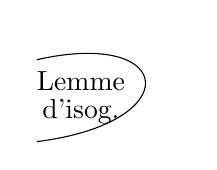
\begin{tikzpicture}[scale=.8]
\node at (0,0) {\shortstack{\unsure{Lemme}\\\unsure{d'isog.}}};
\draw (-.7,.6) .. controls (1.5,1.1) and (1.7,-.4) .. (-.7,-.7);
\end{tikzpicture}}}
donc $\nu_1^{\unsure{*}}$ et $\nu'_1$ sont \deleted{Alb-équi.} \inserted{de degré $0$ et} tels que les $S_{T\times T'}$ sont nuls. D'autre part, on voit de suite que
\[
Z_1(\nu_1)=Z(\nu),\quad Z'(\nu'_1)=Z'(\nu'),
\]
\deleted{donc on est} d'autre part
\[
Z_1(\nu'_1)=Z(\operatorname{pr}_{1*}(\nu'_1))=0
\]
car $\operatorname{pr}_{1*}(\nu'_1)=0$, sous réserve que $Z$ a été choisi tel que $Z(a)$ soit défini. On a de $=$, si $a'$ est choisi convenablement, $Z'_1(\nu_1)=0$.

On pose donc
\[
Z_2=Z_1+Z'_1,\qquad\nu_2=\nu_1+\nu'_1,
\]
et on aura
\[
Z_2(\nu_2)=z+z'.
\]
\deleted{\unsure{et}} Donc $N(X)$ est bien un \unsure{k-groupe|s-groupe} de $X$.

\margin{\diagram{\begin{tikzcd}[ampersand replacement=\&]
X\times T\arrow[d,dash] \& X\times T\times T'\arrow[l,dash]\arrow[d,dash]\\
T \& T\times T'\arrow[l,dash]
\end{tikzcd}}}

\mspage{25}


\scanpage{27}
Le fait qu'il soit gradué est immédiat. Il contient le groupe des cycles lin. équiv. à $0$, comme il résulte aussitôt des définitions, et du fait que sur $T=\mathbb P^1$, tout $0$-cycle $\nu$ de degré $0$ satisfait $S_T(\nu)=0$. \deleted{Ainsi $N(X)$ est bien un \unsure{k-groupe|s-groupe} de $X$, contenant}

Pour prouver (iii), notons $z$ un cycle de la classe envisagée dans $A^*(Y)$, et considérons un $Z$ sur $Y\times T$ et un $\nu$ comme dans 1.1., donc $z=Z(\nu)$. Si nous changeons $Z,\nu$ dans leur classe d'équivalence linéaire \inserted{en $Z',\nu'$}, $Z'(\nu')$ sera linéairement équivalent à $z$, et le Pb est le $=$ pr $z$ et $z'$. Il suffit maintenant de prouver \deleted{\unsure{et}} qu'il existe $Z',\nu'$ tels que $(f\times\operatorname{id}_T)^*(Z')=Z'_1$ et $Z'(\nu')$, \deleted{$Z'_1(\nu')$} soient définis; en effet, en vertu de la théorie des intersections, on aura alors
\[
f^*(Z'(\nu'))=\deleted{\unsure{f^*}}Z_1(\nu'),
\]
or le premier \unsure{mb.} \deleted{\unsure{représente est dans le}} représente $f^*(z)$ dans $A^*(X)$, \deleted{le deuxième est}

\margin{\diagram{\begin{tikzcd}[ampersand replacement=\&]
X\arrow[r,dash,"{\unsure{-|\to}}" description]\&Y
\end{tikzcd}}}
\margin{\diagram{\begin{tikzcd}[ampersand replacement=\&]
X\times T\arrow[rr,Leftrightarrow,"{\unsure{\Leftrightarrow|\Rightarrow}}" description]\arrow[dr]\& \&Y\times T\arrow[dl]\\
\&\deleted{\unsure{T}}T\&
\end{tikzcd}}}

\mspage{26}


\scanpage{28}
\margin{\uline{à vérifier}}

Nous laissons ici les détails de la vérification de l'existence de $Z',\nu'$.

On prouve (ii) pr \deleted{\unsure{la|les}} \inserted{$=$} méthode que (i), \deleted{\unsure{à nouveau}} en se ramenant au cas où $z,z'$ sont définis en termes des $=$ $T,\nu$ et deux cycles $Z,Z'$ sur $T$. On \inserted{peut} se ramener aussi à (iii) et à l'énoncé analogue à (ii) pr les produits \uline{extérieurs}, ce qui dispense de faire encore bouger les cycles.

La démonstration de (iv) se fait pr l'\unsure{AQT}. Celle de (v) est triviale sur les définitions (ou sur le formalisme de l'équiv. alg.)

\margin{\figure{\begin{tikzpicture}\draw (0,0)--(0,3);\end{tikzpicture}}}

\deleted{\uline{Théorème}} \uline{\unsure{Scholie|Scolie}} 1.3. Les $A'^*(X)$, pr $X$ variable, ont les $=$s propriétés formelles générales que les $A^*(X)$. En particulier, on a la formule de projection, Dans les cas où équiv. linéaire $=$ équiv. Alg. sur $X$ (p. ex. \unsure{l'espace} ponctuel, les $\mathbb P^n$, les variétés de drapeaux) \unsure{ils sont} $=$ équiv. alb.

\mspage{27}


\scanpage{29}
\margin{Ici il semble \unsure{qu'on utilise} le fait que dans 1.1. on prend \(T\) \uline{projectif}}
\uuline{Théorème} 1.4. Soit \(X\) projective lisse connexe de dim \(n\) sur \(k\). \deleted{Alors pr les cycles de dim 0 et pr les cycles de codim 1, l'équiv.}

(i) Soit \(\nu\) un 0-cycle sur \(X\). Alors \(\nu\) est alb. équiv. à 0 ssi \(\nu\) est de degré 0, et \(S_X(\nu)=0\).

(ii) Soit \(D\) un diviseur sur \(X\). Alors \(D\) est alb-équi. à 0 ssi \(D\) est lin. équivalent à 0.

\margin{\uline{Remarque} 1.5. On ignore, \inserted{déjà} pr les 0-cycles, si l'équiv. d'Alb. est identique à l'équivalence linéaire. (Vrai pr tous les cycles???).}

\uuline{Démonstration}. (i) Si \(\nu\) est de degré 0 et \(S_X(\nu)=0\), on a \(\nu\) alb-équi. à 0 pr définition [prendre \(T=X\), \(Z=\text{diagonale de }X\), donc \(\nu=Z(\nu)\)]. L'assertion en sens inverse résulte de [\hspace{1em}, 1.2.]. Pour (ii), on sait déjà que lin. équi. à \(0\Rightarrow\) alb-équi. à 0, prouvons le sens inverse. On doit prouver que si
\mspage{28}


\scanpage{30}
\(Z\) est un diviseur sur \(X\times T\) et \(\nu\) sur \(T\) est de degré 0 et tel que \(S_T(\nu)=0\), alors \(Z(\nu)\) est lin. équi. à 0. Or \(\unsure{\operatorname{cl}}Z(\nu)=u(S_T(\nu))\), où \(u:\deleted{\unsure{\operatorname{Alb}}}\ A_T\longrightarrow\underline{\operatorname{Pic}}_X^0\) est l'hom défini pr \(Z\).

\uline{Théorème} 1.\deleted{\unsure{5}}\inserted{6}. Soient \(z,z'\) deux classes dans \(A'{}^*(X)\) alg. équiv. à 0, \(X\) étant \deleted{[projective]}\inserted{\unsure{qu. pr.}}. Alors \(zz'=0\). \inserted{[Si \(X\) est projective, alors il suffit que l'un des facteurs \(z\) soit alg. équiv. à 0, et l'autre \uline{num.} équiv. à 0??]}
\margin{\deleted{À voir si \unsure{il ne suffit pas} \unsure{que pour} \(z\) ou \(z'\) on \unsure{sait} que \unsure{\(\tau\)-équiv.|\(\simeq\)-équiv.} à 0, voire si \(X\) \unsure{n'est pas} \unsure{linéaire|qu. pr.}}}
\margin{\figure{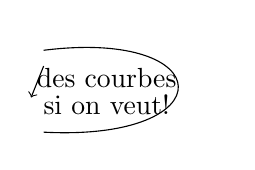
\begin{tikzpicture}[scale=.8]
\node at (0,0) {\shortstack{\unsure{des courbes}\\si on veut!}};
\draw (-1,.65) .. controls (1.8,1) and (1.9,-.8) .. (-1,-.65);
\draw[->] (-1,.4)--(-1.2,-.1);
\end{tikzpicture}}}

\deleted{\unsure{Cela}} \inserted{La première assertion} résulte formellement de la définition de ``alg. équiv. à 0'' \inserted{(via variétés \(T\) \uline{projectives} \uline{lisses} connexes)} et du fait que si \(T,T'\) sont deux \inserted{telles} variétés, \deleted{et} (leur connexité suffit) et \(x,y\) sont deux points de \(T\), \(x'\) et \(y'\) deux pts de \(T'\), alors
\[
\nu=\inserted{((x)-(y))\times((x')-(y'))=}(x,x')-(x,y')-(y,x')+(y,y')
\]
est tel que \(\deleted{\unsure{\nu\in A}}\ S_{T\times T'}(\nu)=0\).
\margin{NB. On ignore si cet \(\nu\) est \uline{lin.} équiv. à 0, $=$ si \(T,T'\) sont des \uline{courbes}!}

[Il y a intérêt à transformer \deleted{le Pb} \inserted{l'énoncé} en un énoncé sur l'opération \(\times\).]
\mspage{29}


\scanpage{31}
2. \uline{Familles de classes de cycles \deleted{\unsure{à équiv.}} \inserted{mod équiv. d'Alb.}}

\uline{Théorème} 2.1. Soient \(X^n\) et \(Y^m\) comme d'habitude, et \(Z\in\deleted{\unsure{\operatorname{Cy}}}A^i_{\inserted{\text{\textcircled{alb}}}}(X\times Y)\), d'où une \deleted{homomorphisme}\inserted{application} \(\nu\longmapsto Z(\nu)\) de \(\deleted{\unsure{A_0(Y)}}\inserted{A_{0\,\mathrm{alb}}(Y)}\) dans \(A^i_{\mathrm{alb}}(X)\).
\deleted{Il existe une application et une seule de \((A^0_{\mathrm{alb}}(Y)\simeq\operatorname{Alb}_Y^*(k))\) dans \(A^i_{\mathrm{alb}}(X)\) telle que pour tout \(\nu\in\unsure{\operatorname{Alg}}_0(Y)\)}
Or \(A_{0\,\mathrm{alb}}(Y)\overset{S_Y}{\simeq}\deleted{\unsure{B}}A_Y^*(k)\), d'où un hom de groupes
\diagram{\begin{tikzcd}[ampersand replacement=\&,execute at end picture={\draw ([xshift=3mm]ay.west) ellipse (3mm and 4mm);\node at ([xshift=3mm,yshift=-6mm]ay.west) {Alb};}]
|[alias=ay,label={left:$u_Z^*:\,$}]| A_Y^*(k)\arrow[r]\&A^i_{\mathrm{alb}}(X)
\end{tikzcd}}
\deleted{dont la restriction à \(A_Y^{(n)}(k)\) est} défini pr la condition
\[
\deleted{\unsure{S_Y}}Z(\nu)=u_Z(S(\nu))
\]
pr tt \(\nu\) (resp. pr tt \(\nu\) de degré \(n\), si on regarde la restriction en degré \(n\)).

\uline{De plus}, si on regarde l'hom \uline{induit} sur \(A_Y(k)=A_Y^0(k)\)
\[
u_Z:A_Y(k)\longrightarrow A^i_{\mathrm{alb}}(X),
\]
on a ce qui suit : \deleted{Il existe un hom de passage de VA \(\varphi:A'\longrightarrow A_Y\) et un cycle \(Z'\in A^i_{\mathrm{alb}}(\,\unsure{/}\)}

(i) Il ne dépend que de la classe de \(Z\) dans \(A^{i\,\unsure{\tau}}_{\deleted{\unsure{\mathrm{alg}}}}(X\times Y)\)
\margin{[À \unsure{réserver} pr plus tard}

(ii) Il existe une \deleted{hom}\inserted{isogénie}
\mspage{30}


\scanpage{32}
\margin{\figure{\begin{tikzpicture}\draw (0,.1)--(.1,0)--(1,.7);\end{tikzpicture}}}
de VA
\[
\varphi:A'\longrightarrow A_Y
\]
et un \(Z'\in A^i_{\mathrm{alb}}(\unsure{X}\times A')\), \deleted{\unsure{et}} tel que \(Z'((0))=0\) (ou ce qui revient au \(=\), tel que l'application \(v_{Z'}:\deleted{\unsure{a}}a'\leadsto Z'(a')\) de \(A'\) dans \(\deleted{\unsure{\operatorname{Alb}_Z}}\figure{\begin{tikzpicture}[baseline=(cycle.base)]\node[draw,ellipse,inner sep=2pt] (cycle) {$A^i_{\mathrm{alb}}(X)$};\end{tikzpicture}}\) soit un hom de groupes) tel que
\margin{diviseur de degré 1 concentré en 0}
\[
u_Z\circ\varphi(k)=v_{Z'}
\]

\uline{Dém}. Supposons qu'il existe un cycle \deleted{\unsure{Z}} \(U\) sur \(Y\times A_Y\), de codim \(m\), tel que pr tt \(a\in A_Y\), on ait \(S_Y(U(a))=a\). Alors la ``famille algébrique de \unsure{diviseurs}'' composée \(a\leadsto Z(U(a))=Z'(a)\) convient : \unsure{le § entraîne} que pr tt \(\nu\in\deleted{\unsure{\operatorname{Alb}}}A_{0\,\mathrm{alb}}(Y)\) \inserted{de degré 0,} on aura
\[
\deleted{\unsure{\operatorname{cl}}Z'(a).}
\qquad Z(\nu)=Z'(S(\nu))
\]
\deleted{\unsure{et que} \(\nu\) est de}
Car pr le voir, on \deleted{peut \unsure{remplacer} \(\nu\) \unsure{par un}} \inserted{le \unsure{cycle} \(U(a)\), \unsure{dont il faut vérifier}}
\deleted{\unsure{cycle} \(\nu\) \unsure{est équivalent à}}
\[
\begin{aligned}
Z(U(a))&=Z'(S(U(a))\phantom{)}\\
&\Vert\\
&Z'(a)
\end{aligned}
\qquad\text{O.K.}
\]
Mais \deleted{à priori} on ne sait pas si on peut
\mspage{31}


\scanpage{33}
trouver \(U\) \inserted{comme ci-dessus}, mais on peut trouver \(U\) de façon que l'on ait
\[
S_Y(U(a))=na
\]
alors, posant \(Z'(a)=Z(U(a))\), la relation
\[
Z'(S_Y(\nu))=nZ(\nu)
\]
\margin{\(\nu\) de degré 0 sur \(Y\).}
\deleted{Car on peut \unsure{écrire} \(nS(\nu)=U(a)\) où \(a=S_Y(\nu)\), \(S(\nu)\) de la forme \(U(a')\), car si \(a'=S_Y(\nu)\), on aura \(S_Y(U(a'))=na'=S_Y(n\nu)\) donc \(U(a')=n\nu\), et comme on aura \(a'=na\) pr \unsure{convenable} \(n\), il s'ensuivra \(U(a)\)}

Pour le voir, soit \(a=S_Y(\nu)\), on aura
\[
\deleted{\unsure{\operatorname{cl}Z'}}S_Y(U(a))=na=S_Y(n\nu)
\]
d'où \(\deleted{U(a)=n\nu,}\inserted{U(a)\unsure{=|\equiv}n\nu}\)
d'autre part on aura
\[
\begin{array}{ccc}
\deleted{\unsure{\operatorname{cl}}}Z'(S_Y(U(a)))&=&nZ(U(a))\\
\Vert&&\Vert\\
Z'(na)&&nZ'(a)
\end{array}
\]
\deleted{d'où, comme \(U(a)=n\nu\)}
\[
\deleted{nZ'(S_Y(\nu))=n^2Z(\nu)}
\]
Or tout élément de \(A_{0\,\mathrm{alb}}(Y)\) de degré 0 est de la forme \(n\unsure{\zeta}\) (car \(A_Y(k)\) est divisible!) donc appliquant ce qui précède à \(\unsure{\zeta}\) au lieu de \(\nu\), on trouve
\[
Z'(S_Y(\nu))=nZ(\nu).
\]
On prend comme isogénie la multiplication pr \(n\).
\mspage{32}


\scanpage{34}
Cela prouve (ii). Pour (i), on note qu'on sait déjà que si \(Z\) est alg. équiv. à 0, alors l'hom correspondant \(u:A_Y(k)\longrightarrow A^i_{\mathrm{alb}}(X)\) est nulle (Th. 1.6.), donc si \(Z\) est \(\tau\)-équivalent à 0, alors l'hom \(u\) est tel que \(mu=0\) pour quelque \(m>0\), donc \(u=0\) car \(A_Y(k)\) est \(m\)-divisible.

\uline{Corollaire} \unsure{2.7|2.2}. Pour qu'un cycle algébrique de codim \(i\) sur \(X\) soit alg. équiv. à 0, il f. et s. qu'il soit Albanese-équivalent à un diviseur de la forme \(Z(a_0)\), où \deleted{\(A\) est \unsure{une}} \(Z\) est un cycle de codim \(i\) sur un \deleted{VA \(A\),} produit \(A\times X\), \(A\) une variété abélienne, tel que \(\deleted{\unsure{\operatorname{Alb}}}a\leadsto Z(a):A\longrightarrow\deleted{\unsure{Z}}A^i_{\mathrm{alb}}(X)\) soit un hom de groupes.

\uline{Corollaire} 2.3. Pour tt entier \(n>0\), le groupe \(P^i(X)\) des \deleted{classes d'\unsure{équivalence}, à équiv. d'Alb.}\inserted{\(A^i_{\mathrm{alb}}(X)\), formé des classes de cycles} alg. équiv. à 0, est \(n\) \uline{divisible}.

\uline{Corollaire} 2.4. Soient \(Z,Z'\in A^*_{\mathrm{alb}}(X)\), dont l'un est alg. équiv. à 0 et l'autre \(\tau\)-équiv. à 0. Alors \(ZZ'=0\).
\mspage{33}


\scanpage{35}
\uline{Définition} 2.5. Soient \(X,Y\ldots\) et considérons une application
\diagram{\begin{tikzcd}[ampersand replacement=\&]
\varphi:\uline{Y(k)}\arrow[r]\&|[draw,ellipse]|A^i_{\mathrm{alb}}(X)
\end{tikzcd}}
On dit que cette application est \uline{algébrique} si

1°) L'hom \(\deleted{\unsure{Z}}\operatorname{Cyc}_0(Y)\longrightarrow A^i_{\mathrm{alb}}(X)\) correspondant se factorise pr \(\deleted{A}A_{0\,\mathrm{alb}}(Y)\simeq A_Y^*(k)\), i.e. \deleted{\unsure{elle}} est nulle sur les \(\nu\) de degré 0 tels que \figure{\begin{tikzpicture}[baseline=(sy.base)]\node[draw,ellipse,inner sep=2pt] (sy) {$S_Y(\nu)=0$};\end{tikzpicture}}.
\margin{\diagram{\begin{tikzcd}[ampersand replacement=\&]Y\arrow[r]\&A_Y^1\arrow[r,"N"]\&A_Y^N\end{tikzcd}}}

2°) L'hom induit
\diagram{\begin{tikzcd}[ampersand replacement=\&]
|[draw,ellipse,label={left:$\varphi:\,$}]|A_Y^{\unsure{0|*}}(k)\arrow[r]\&A^i_{\mathrm{alb}}(X)
\end{tikzcd}}
est tel que pr \(N>0\) convenable, \(\underline{N\varphi}(x)=\varphi(Nx)\) pourra être induit pr un cycle algébrique
\[
Z\in A^i_{\mathrm{alb}}(X\times A_Y)
\]

\uline{Prop.} 2.6. Si \(\varphi\) est définie pr un \(Z\in A^i_{\mathrm{alb}}(X\times Y)\), elle est \uline{algébrique}.

C'est 2.1.
\margin{Va être généralisé en 2.7. (ii)}

\uline{Prop.} 2.7. \inserted{(0) Forment un \uline{\unsure{k-groupe|s-groupe}}. Si \(N\varphi\) est alg., \(\varphi\) l'est.}

(i) Fonctorialité en \(Y\). \deleted{Alors \unsure{\(\varphi\) induit}}

(ii) Fonctorialité en \(X\), plus gén., si on a un hom \(A^i_{\mathrm{alb}}(X)\longrightarrow A^{\unsure{j}}_{\mathrm{alb}}(X')\) défini pr une classe de correspondances algébriques \uline{à coeff.} \deleted{\uline{\unsure{rationnels}}} entiers.
\mspage{34}


\scanpage{36}
N.B. Fixons un pt \(y_0\) de \(Y\). Alors le gr des familles algébriques \(Y(k)\mathbin{-}A^i_{\mathrm{alb}}(X)\) est isom à \(A^i_{\mathrm{alb}}(X)\times\operatorname{Hom\,alg}(A_Y,A^i_{\mathrm{alb}}(X))\), où le dernier facteur désigne les familles algébriques qui sont des hom de groupes, i.e. nulles à l'origine. On peut donc se limiter à étudier les hom ``alg.'' \(A_{\deleted{\unsure{Y}}}(k)\mathbin{-}\figure{\begin{tikzpicture}[baseline=(target.base)]\node[draw,ellipse,inner sep=2pt] (target) {$A^i_{\mathrm{alb}}(X)$};\end{tikzpicture}}\), \inserted{où \(A\) est une VA,} et, interprétant \(A\) comme
\[
A_{0\,\mathrm{alb}}(A)=A^\alpha_{\mathrm{alb}}(A)^{(\mathrm{alg.\,équiv.\,0})}\qquad(\alpha=\dim A)
\]
on peut considérer \deleted{\unsure{le}} ces objets comme des cas particuliers des \uline{homs algébriques}
\[
\varphi:P^j(X')\mathbin{-}P^i(X).
\]
\margin{\diagram{\begin{tikzcd}[ampersand replacement=\&]A(k)\simeq P^{\unsure{\alpha|n}}(A)\arrow[r]\&P^i(X)\end{tikzcd}}}
Un hom de groupes \(\varphi\) est dit ``algébrique'' s'il existe un entier \(N>0\) tel que \(N\varphi\) soit définissable pr un cycle algébrique sur \(\unsure{X\times Y'|X\times X'}\).

(Alors \(\varphi\) sera définissable pr un cycle alg. à coeff \uline{rationnels} --- mais attention, un cycle à coeff rationnels \uline{quelconque} ne définit pas en général un hom \(P^j(X')\mathbin{-}P^i(X)\), \(=\) si les degrés sont les bons\ldots.). Ces homs \uline{se composent}
\mspage{35}


\scanpage{37}
\margin{?\quad\figure{\begin{tikzpicture}\draw (0,0)--(0,1.4);\end{tikzpicture}}}
Une question plus subtile est s'ils peuvent s'inverser, quand c'est des isomorphismes\ldots.

\uline{Dualité} entre \(P^i(X)\) et \(P^{\deleted{n+1-i}\inserted{j}}(X)\) \inserted{pr \(i+j=n+1\)} : Si \(A,B\) \deleted{\unsure{les}} \deleted{\unsure{unes}}\inserted{des} VA, \deleted{dont la dualité est} accouplées pr une dualité parfaite \((A\simeq\unsure{B'|B^*},B\simeq A^*)\), alors il y a correspondance biunivoque entre \(\operatorname{Hom\,alg}(A,P^i(X))\) et \(\operatorname{Hom\,alg}(P^{\unsure{j|1}}(X),B)\).

En effet, si on a un hom \(A\longrightarrow P^i(X)\), défini pr un \(Z\in A^i_{\mathrm{alb}}(X\times A)\), alors \({}^tZ\) définit un hom
\diagram{\begin{tikzcd}[ampersand replacement=\&]
P^j(X)\arrow[r]\&P^{i+j-n}(A)=P^1(A)\arrow[d,phantom,"\simeq" rotate=90]\\
\&B
\end{tikzcd}}
et inversement si on a \(P^j(X)\longrightarrow B\). \deleted{Notations}\inserted{Cependant,}
\deleted{\(\unsure{{}^t\varphi=\varphi^t}\). Plus généralement}
il faut vérifier que \(P^j(X)\longrightarrow B\) ne dépend que de l'\uline{application} \(A\longrightarrow P^i(X)\), pas du cycle \(Z\).
\margin{\figure{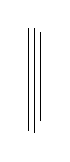
\begin{tikzpicture}[x=1cm,y=1cm]\draw (0,0)--(0,1.3);\draw (.08,-.03)--(.08,1.3);\draw (.16,.12)--(.16,1.25);\end{tikzpicture}}}

Question de transposition se pose, plus généralement, pr \(P^i(X)\mathbin{-}P^{i'}(X')\) en \(P^{j'}(X')\mathbin{-}P^j(X)\).

Cf plus bas\ldots.
\mspage{36}


\scanpage{38}
3. Homomorphisme \(\ell\)-adique associé à une \deleted{\unsure{hom}} famille abélienne de cycles.

Soit \(A\) une V.A., \(Z\in A^i_{\mathrm{alb}}(X\times A)\), d'où
\[
\deleted{\unsure{\varphi=}}u_Z:A(k)\longrightarrow A^i_{\mathrm{alb}}(X)
\]
mais aussi
\[
a({}^tZ):H^{2(n-i)+1}(X)(n-i)\longrightarrow H^1(A)
\]
(coefficients \(\ell\)-adiques \(\deleted{\unsure{\mathbb Q}}\mathbb Z_\ell\)). Je dis que mod. torsion (i.e. à coefficients \(\mathbb Q_\ell\)!) cet homomorphisme ne dépend que de \(u_Z\), pas de \(Z\), \deleted{\unsure{donc}} et de façon précise que

\figure{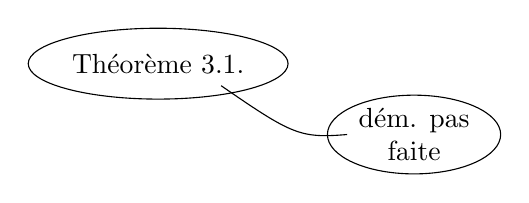
\begin{tikzpicture}[x=1cm,y=1cm]
\node at (0,0) {\uline{Théorème} 3.1.};\draw (0,0) ellipse (1.65 and .45);
\draw (.8,-.28) .. controls (1.7,-.9) and (1.8,-.95) .. (2.4,-.9);
\draw (3.25,-.9) ellipse (1.1 and .5);\node[align=center] at (3.25,-.9) {dém. pas\\faite};
\end{tikzpicture}}
\diagram{\begin{tikzcd}[ampersand replacement=\&,column sep=large,execute at end picture={\node at ([xshift=2mm]hyp.east) {$\unsure{<|\Longleftarrow}$};}]
|[alias=hyp]|u_Z=0\arrow[r,Rightarrow,"?"]\&a({}^tZ):H^{(n-i)+1}\mathbin{-}H^1\text{ est nul}
\end{tikzcd}}
\margin{?\quad A-t-on une réciproque}

\uline{Démonstration}. Choisissons une ``courbe ample'' \(C\) sur \(A\), \deleted{\unsure{d'ici alors}} d'où \(C\longrightarrow A\) induit
\diagram{\begin{tikzcd}[ampersand replacement=\&]
\deleted{C\times X\mathbin{-}}\inserted{X\times C}\arrow[r]\&\deleted{A_C\longrightarrow A}\inserted{X\times A}
\end{tikzcd}}
d'où \(Z'\in A^i_{\mathrm{alb}}(C\times X)\) et pr conséquent
\[
u_{Z'}:C(k)\longrightarrow A^i_{\mathrm{alb}}(X)
\]
\[
a({}^tZ'):H^{2(n-i)+\unsure{3|1}}\deleted{(\unsure{X})}(n-i)\mathbin{-}H^1(C)
\]
et comme \(H^1(A)\mathbin{-}H^1(C)\) est injectif, \(C(k)\mathbin{-}A(k)\) surjectif, on a
\mspage{37}


\scanpage{39}
\[
u_Z=0\quad\unsure{\Longleftarrow|\Longleftrightarrow}\quad u_{Z'}=0
\]
\[
a({}^tZ)=0\quad\Longleftrightarrow\quad a({}^tZ')=0
\]
On est donc ramené à la question analogue, avec \(A\) remplacé pr \(C\). Or \deleted{tout} \deleted{cycle} la décomposition
\[
H^N(X\times C)\simeq H^N(X)\otimes H^0(C)+H^{N-1}(X)\otimes H^1(C)+H^{\unsure{N-2|N-1}}(X)\otimes H^{\unsure{2|1}}(\unsure{C}
\]
est algébrique, comme \deleted{\unsure{on}} on vérifie aisément. Appliquant ceci au cas \(N=2i\), et notant qu'un cycle algébrique appartenant à l'un des deux facteurs extrêmes donne un \(u_{Z'}\) \uline{et} un \(a({}^tZ)\) nul, on est ramené au cas d'un cycle appartenant au facteur médian, i.e. dont la \uline{projection} sur \(X\), et la ``restriction'' à \(X\), sont nulles.
\mspage{38}


\scanpage{40}
Astuce de Tate

sur les cycles

décomposables

\mspage{39}


\scanpage{41}
Soit $A$ une VA sur $k$ alg. clos, d'où module $\mathbb{T}_\ell(A)$ \deleted{$\unsure{\otimes}$} sur la pro-alg. de Lie \deleted{$\unsure{\mathfrak{g}_\ell}$} $\mathfrak{g}(k)=\mathfrak{g}$.

Soit $K$ une clôture alg. de $\mathbb{Q}_\ell$, posant
\[
\mathbb{T}_K(A)=\mathbb{T}_\ell(A)
\]
de sorte que $\mathbb{T}_K(A)$ est un module sur $\mathfrak{g}\otimes_{\mathbb{Q}_\ell}K=\mathfrak{g}_K$. Supposons

a) La \deleted{\unsure{les}} conj de Tate vérifiée pr $H^2(A,\mathbb{Q}_\ell(1))$
\[
H^2(A\deleted{\unsure{\times}},\mathbb{Q}_\ell(1))^{\mathrm{alg}}
=H^2(A,\mathbb{Q}_\ell(1))^{\mathfrak{g}}
\]

b) $\mathfrak{g}_K$ opérant sur \deleted{$\unsure{\mathfrak{g}}$ est} $\mathbb{T}_K(A)$ est ``\unsure{pseudoalgébrique}''

[i.e. les valeurs propres des frobénius \deleted{\unsure{sont}} de norme $q$ sont $\varepsilon q^{-1/2}$, $\varepsilon$ une racine de l'unité\ldots]

\margin{\unsure{Pr. Tits}, le premier cas est un cas particulier du second}

\uline{ou} $\mathbb{T}_K(A)$ se décompose en deux morceaux $V_1\times V_2$, tels que chacun soit propre pr ``presque tous'' les Frobénius, avec des valeurs propres différentes pr presque tous les Frobénius.

[Ces conditions sont remplies si $A$ est une \deleted{produit}\inserted{puissance} \margin{$C^n$} d'une \deleted{de} courbe elliptique \inserted{$C$ définissable} sur un corps fini $\mathbb{F}_q$, comme on voit en notant que a) \deleted{\unsure{et b)} \unsure{triviale|triviales} \unsure{se réduit pr passage à une puiss.|se déduit pr passage à une puiss.} \unsure{adéquate, et pr lequel b) est}} a été vérifié pr Mumford. Ceci est connu.

\mspage{40}


\scanpage{42}
au cas du produit de \uline{deux} courbes elliptiques), et b) est trivial à partir du cas de $C$, car b) est stable pr \deleted{produit} puissances cartésiennes]. Alors on a pour tt $i$
\[
D^{2i}(A,\mathbb{Q}_\ell(i))
=H^{2i}(A,\mathbb{Q}_\ell(i))^{\mathrm{alg}}
=H^{2i}(A,\unsure{\mathbb{Q}_\ell i)|\mathbb{Q}_\ell(i)})^{\mathfrak{g}}
\]
\margin{décomposables $\mathbb{Q}_\ell$-algébriques)}

En effet, \deleted{l'hypothèse} à priori on a les inclusions $\subset$, $\subset$, et l'hypothèse implique l'égalité des extrêmes\ldots

\mspage{41}


\scanpage{44}
27.8.65

Mon Cher Serre,

Je continue à retourner dans tous les sens les questions de cycles algébriques; techniquement parlant je vois la question plus clairement, mais cependant il manque toujours le pas décisif. Comme je te connais allergique à la cohomologie, j'ai envie de t'énoncer les deux conjectures-clef, qu'il s'agit de démontrer, de façon purement géométrique i.e. sans parler de cohomologie. $X$ désigne une variété projective lisse connexe sur le corps algébriquement clos $k$, de dimension $n$, $Y$ une section hyperplane lisse. Par $C^i(X)$ je désigne le groupe des classes de cycles de codimension $i$ mod équivalence algébrique, tensorisé par $\underline{Q}$, par $\xi\in C^1(X)$ la classe de $Y$

\uline{Conjecture} A Pour tout entier $i$ tel que $2i\leq n$, le produit par $\xi^{n-2i}$ induit un isomorphisme $C^i(X)\xrightarrow{\sim}C^{n-i}(X)$.

Modulo vérification que je n'ai pas écrite en détail, il suffit même dans cette conjecture de vérifier la surjectivité, et de le faire pour $n=2i+1$. Le premier cas qui échappe pour le moment est $i=1,n=3$. Cette conjecture implique l'analogue, pour les $C^i$, des théorèmes connus de Lefschetz sur la comparaison de la cohomologie de $X$ et de $Y$ par les homomorphismes d'image directe et d'image inverse (pour la formulation correcte, se rappeler seulement que $C^i$ devient $H^{2i}$), en même temps qu'il implique les théorèmes de Lefschetz cohomologiques eux-mêmes, dont la forme formellement la plus forte consiste à affirmer que $\xi^{n-i}$ induit un isomorphisme de $H^i$ et $H^{2n-i}$ pour la cohomologie à coefficients $\underline{Q}_\ell$; je te signale que ce théorème purement cohomologique n'est pas même démontré pour le moment ! N'est démontré que le théorème de Lefschetz ``faible'' affirmant que la dimension cohomologique d'une variété affine de dimension $n$ est majorée par $n$, ce qui pour la variété affine $U=X-Y$ prend la forme : $H^i(X)\longrightarrow H^i(Y)$ est bijectif pour $i\leq n-2$, injectif pour $i=n-1$, ou encore : $H^i(Y)\longrightarrow H^{i+2}(X)$ est bijectif pour

\hfill $\ldots/\ldots$

\mspage{43}
